%
\documentclass[12pt, oneside]{report}
\usepackage[margin=0.85in]{geometry}
\linespread{1}
\usepackage{xcolor}
\usepackage[colorlinks=false, linkbordercolor=white, citebordercolor=white, 
    filebordercolor=white, urlbordercolor=white]{hyperref}
    
\usepackage{graphicx}
\usepackage[utf8]{inputenc}
\usepackage[T1]{fontenc}
\usepackage[spanish]{babel} 

\usepackage{fancyhdr}\setlength{\headheight}{14.49998pt}
\pagestyle{fancy}
\renewcommand{\headrulewidth}{0.4pt}
\fancyhead{}
\fancyhead[L]{Estructuras de Datos Avanzadas - 2024-1 - Tarea 1}

\fancyhead[R]{<Tu nombre aquí>}
\fancyfoot[C]{\thepage}

\usepackage{titlesec}
\titlespacing{\chapter}{0pt}{*4}{*2.5}

\titleformat{\chapter}{\normalfont\huge\bf}{\thechapter}{20pt}{\huge\bf}


\usepackage{listings}
\definecolor{dgray}{gray}{0.35} 
\definecolor{lgray}{gray}{0.95} 

\lstset{ 
language=python, 
basicstyle=\ttfamily\small, 
backgroundcolor=\color{lgray}, 
commentstyle=\ttfamily\small\itshape\color{dgray}, 
showstringspaces=false, 
numbers=left, 
numberstyle=\ttfamily\small, 
stepnumber=1, 
firstnumber=last, 
breaklines=T} 

\begin{document}

\begin{titlepage}
    \begin{center}
        \vspace*{1cm}
        
        \Huge
          \textbf{Estructuras de Datos Avanzadas}
        \vspace{0.5cm}
        \small
        \\
        \textit{Adriana Ramırez Vigueras}\\
        \textit{Fhernanda Montserrat Romo Olea}\\
        \textit{Marco Antonio Velasco Flores}\\
        \\
        \vspace{0.5cm}
        \LARGE
        Tarea 1
        
        \vspace{1.5cm}
        
        \textbf{<Tu nombre aquí>} 
   		  \vspace{1.5cm}
        
        \textsc{Facultad de Ciencias} 
       
        \vfill
        
        Semestre 2024-1 
        
        \vspace{0.8cm}
          \Large
        \vspace{0.5cm}
       Entrega: 16 Octubre 2023 - 11:59 PM
        
    \end{center}
\end{titlepage}
\addtocontents{toc}{~\hfill\textbf{Page}\par}
\textbf{Pregunta 6}
Decimos que un árbol binario de búsqueda $T_1$ puede ser \textsc{right-converted} a un árbol binario
de búsqueda $T_2$ si es posible obtener $T_2$ de $T_1$ por a tráves de una serie de llamadas a la operación
\textsc{right-rotate}.
\begin{itemize}
\item Da un ejemplo de dos árboles $T_1$ y $T_2$ tal que  $T_1$ no pueda ser \textsc{right-converted} en $T_2$.

\begin{center}
  \begin{figure}[h]
    \centering
    \subfloat[T1]{
      \label{f:T1}
      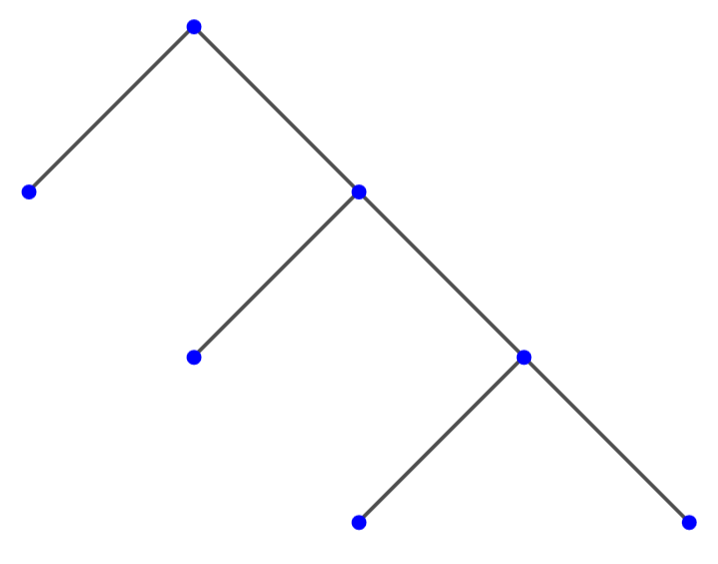
\includegraphics[width=0.4\textwidth]{T1.png}}
    \subfloat[T2]{
      \label{f:T2}
      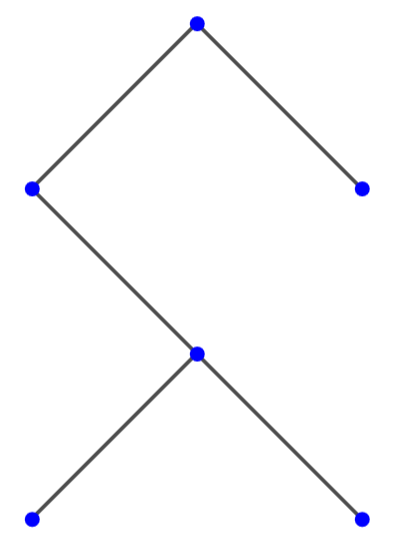
\includegraphics[width=0.25\textwidth]{T2.png}}
    \caption*{Árboles no reducibles por rotación.}
    \label{f:animales}
  \end{figure}


  %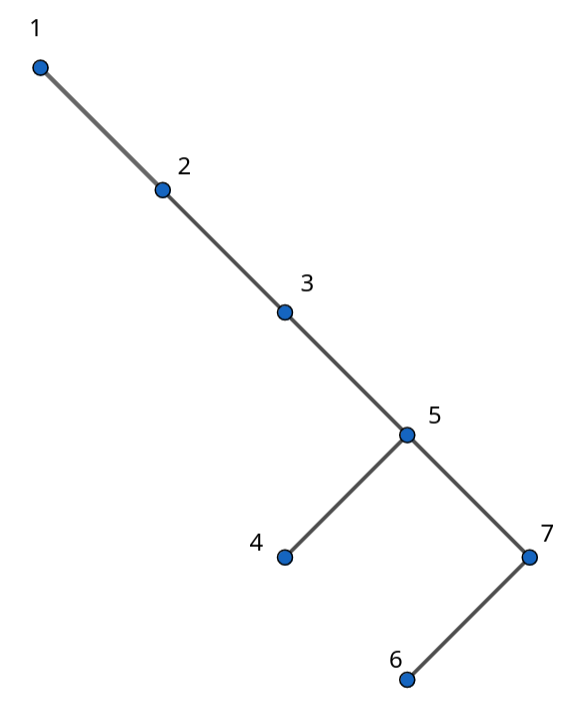
\includegraphics[scale=0.3]{./02.png}
\end{center}


\item Demuestra que si un árbol $T_1$ puede ser \textsc{right-converted} a $T_2$, entonces $T_1$ puede ser
  \textsc{right-converted} usando $O(n^2)$ operaciones \textsc{right-rotate}.\newline

Observemos el peor caso para transformar $T_1$ a $T_2$ por medio de \textsc{right-converted}. Este se da cuándo
$T_2$ es totalmente inverso a $T_1$, esto es, para el vértice raíz rotemos hacia la derecha $n - 1$ veces,
para los nodos hijos rotemos $n - 2$ y $n - 3$ veces de manera respectiva de izquierda a derecha. Si aplicamos
estos pasos de manera iterativa podemos concluir que el número de rotaciones necesarias para transformar $T_1$
en $T_2$ son
\[(n - 1) + (n - 2) + \dotsm + 2 + 1 = \frac{n(n - 1)}{2} \in \mathcal{O}(n^2)\]
por lo que tenemos un orden de rotaciones cuadrático.
\end{itemize} 

\textbf{Pregunta 1.}
%\noindent
Muestra que dado un conjunto $T$ de $n$ nodos $x_1, x_2, \dots, x_n$ con valores y prioridades distintas, el árbol treap asociado a $T$ es único. Hint: utiliza inducción sobre $n$.\newline

\begin{proof}
  Procedamos por inducción en el número de nodos. Observemos que para un nodo

  %%%%%%%%%%%%%%%%%%%%%%%%%%%%%%%%%%%%%%%%%%%%%%%%%%%%%%%%%%%%%%%%%%%%%%%%%% FIGURE 1
  \begin{figure}[ht!]
    \centering
    \begin{tikzpicture}
      %% Primer bloque:
      \node(A) [blueV, label=180:$q$] at (0,0){};
    \end{tikzpicture}
  \end{figure}
  
  se cumple que el árbol Treap asociado a $q$ (en este caso) es
  único.\newline

  Supongamos que para un conjunto $T' = \{q_1, \dotsm, q_k\}$ de tamaño
  $k < n$ con valores y prioridades distintas se cumple que el árbol Treap asociado
  a $T'$ es único\footnote{Hipótesis de inducción.}.\newline

  
\tikzset{
itria/.style={
  draw,dashed,shape border uses incircle,
  isosceles triangle,shape border rotate=90,yshift=-1.45cm},
rtria/.style={
  draw,dashed,shape border uses incircle,
  isosceles triangle,isosceles triangle apex angle=90,
  shape border rotate=-45,yshift=0.2cm,xshift=0.5cm},
ritria/.style={
  draw,dashed,shape border uses incircle,
  isosceles triangle,isosceles triangle apex angle=110,
  shape border rotate=-55,yshift=0.1cm},
letria/.style={
  draw,dashed,shape border uses incircle,
  isosceles triangle,isosceles triangle apex angle=110,
  shape border rotate=235,yshift=0.1cm}
}

\begin{center}
  \begin{tikzpicture}[sibling distance=5cm, level 2/.style={sibling distance =2cm}]
    \node[draw,fill=black] {}
         { node[itria] {$T'$} };
  \end{tikzpicture}
\end{center}

Ahora, observemos que un árbol Treap $T$ de $n$ nodos tiene cómo sub-hijo izquierdo un sub-árbol,
digamos $T_1$, y cómo sub-hijo derecho un sub-árbol, digamos $T_2$. A continuación se muestra un bosquejo
\begin{center}
\begin{tikzpicture}[sibling distance=5cm, level 2/.style={sibling distance =2cm}]
  \node[circle,draw,fill=blue] {}
  child{ node[draw, fill = black] {}
    { node[itria] {$T_1$} } 
  }
    child{ node[draw, fill = black] {}
    { node[itria] {$T_2$} } 
  };
\node[draw] at (3,-5) 
{
\begin{tabular}{cl}
\tikz\node[circle, fill = blue] {}; & Raíz \\
\tikz\node[draw,  fill = black] {}; & Sub-árboles
\end{tabular}
};
\end{tikzpicture}
\end{center}

Podemos notar que $T_1$ y $T_2$ tienen una cantidad de nodos menor que $n$. Por nuestra hipótesis
de inducción $T_1$ y $T_2$ es único, lo que implica que $T$ es único.
\end{proof}
%\subsection*{Respuesta}

%<Tu respuesta aquí>

%\bigskip

\textbf{Pregunta 2}
Se pueden utilizar las estructuras de búsqueda de rangos ortogonales para determinar si un punto particular $(a,b)$ está en un conjunto dado, haciendo una consulta al rango $[a:a] \times [b:b]$.
\begin{enumerate}
   \item Prueba que hacer una consulta así en un árbol $KD$ toma tiempo $O(\log n)$.
   \item ¿Cuál es la complejidad para una consulta así en un árbol de rangos?
\end{enumerate}

$\rhd$ \textbf{Solución:} Para este problema dividamos la solución en dos posibles casos:
\begin{enumerate}
\item[$a$)] Sabemos que hacer una consulta, en un árbol $Kd$, para un rango en
general nos toma $\mathcal{O}(\sqrt{n} + k)$. Sin embargo, consultar un punto
en un árbol $Kd$ sería equivalente a particionar la nuve de puntos por la mitad
y preguntarnos en qué parte queda nuestro punto distinguido, llamemosle $q$. Así,
descartamos aproximadamente la mitad de puntos en dónde no se encuentra $q$. Luego,
subdividimos nuevamente el conjunto de puntos restantes en $2$ y nos preguntamos
en qué parte se encuentra $q$ y podemos descartar la parte en la que no se encuentre.
De esta manera y recursivamente nuestro espacio de búsqueda se reduce a la mitad cada
vez, esto equivale hacer un recorrido de la raíz de nuestro árbol $kd$ hacia las hojas
en búsca del punto $q$. Como cada vez descontamos la mitad del conjunto de puntos
de búsqueda, tenemos la recurrencia $T(n) = 1 + T(\frac{n}{2})$ de manera vértical y
$T(n) = 1 + 2T(\frac{n}{4})$ de manera horizontal, que sabemos que nos genera
un orden logarítmico en base 2 (equivale a bajar por el árbol). Cómo el número de
consultas es igual a $1$, entonces $k = 1 \in \mathcal{O}(1)$. Por tanto, la complejidad
de esta consulta es $\mathcal{O}(\log n)$.
\item[$b$)] En este caso, tenemos una complejidad general de $\mathcal{O}(\log^2 n + k)$,
cómo solo estamos consultando un punto y no un rango, entonces $k = 1 \in \mathcal{O}(1)$.
En la consulta debemos bajar por el árbol hasta encontrar $q.X$ y bajar su árbol ``colgado''
o su árbol asociado en $y$, hacer esto es igual a $\log m$ dónde $m$ es la altura del árbol
asociado con $m \not= n$, pues cada nivel y nodo tiene un árbol compacto de tamaño constante.
Por tanto, la complejidad esta contenida en $\mathcal{O}(\log m \cdot \log n) = \mathcal{O}(\log n)$
con $m$ constante respecto de $n$.

\end{enumerate}
\hfill $\lhd$
%\subsection*{Respuesta}
%<Tu respuesta aquí>


%\bigskip

\textbf{Pregunta 3}
%\noindent
Describe una secuencia de accesos a un árbol splay $T$ de $n$ nodos, con $n \geq 5$ impar, que resulte en $T$
siendo una sola cadena de nodos en la que el camino para bajar en el árbol alterne entre hijo izquierdo e hijo derecho.
\newline

$\rhd$ \textbf{Solución:} Propongamos el siguiente árbol Splay\footnote{Su altura no es logarítmica,
pero sus consultas son amortizadas.}

\begin{center}
  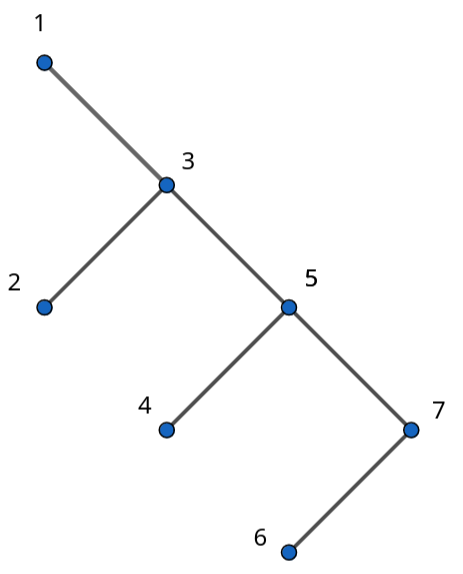
\includegraphics[scale=0.4]{./01.png}
\end{center}

Accedamos a $2$ realizando \code{Zig(2)} seguido de la operación \code{Zag(2)}:
\begin{center}
  \begin{figure}[h]
    \centering
    \subfloat[Zig(2)]{
      \label{f:02}
      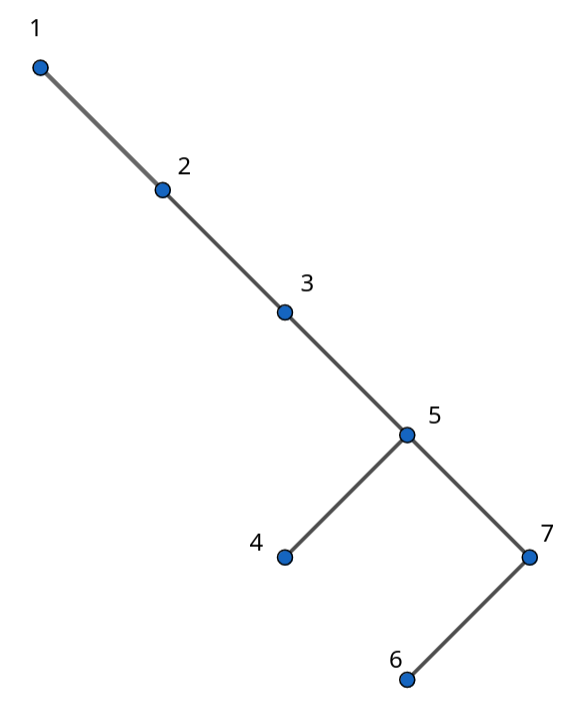
\includegraphics[width=0.4\textwidth]{02.png}}
    \subfloat[Zag(2)]{
      \label{f:03}
      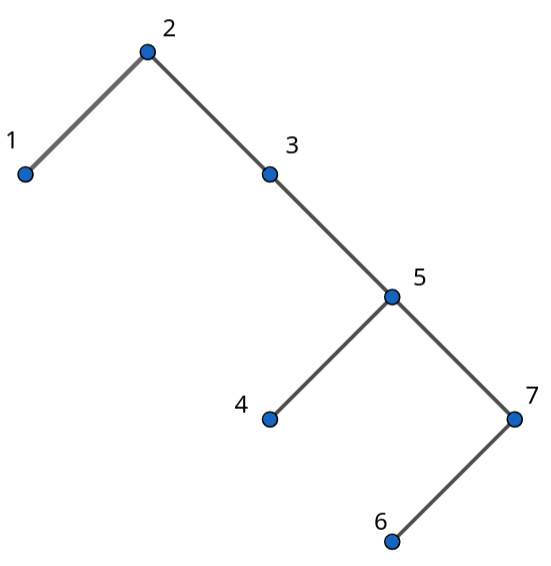
\includegraphics[width=0.4\textwidth]{03.png}}
    \caption*{Acceder a 2.}
    \label{f:animales}
  \end{figure}


  %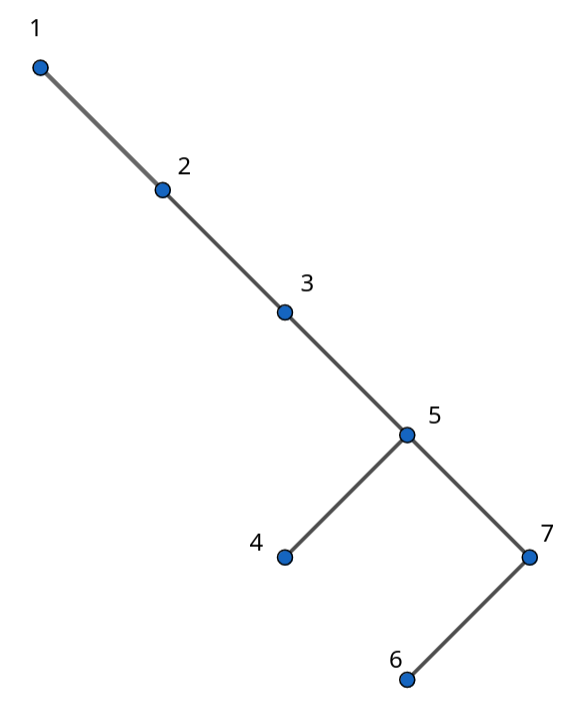
\includegraphics[scale=0.3]{./02.png}
\end{center}

Ahora, accedamos a $3$ realizando un \code{Zag(3)}

\begin{center}
  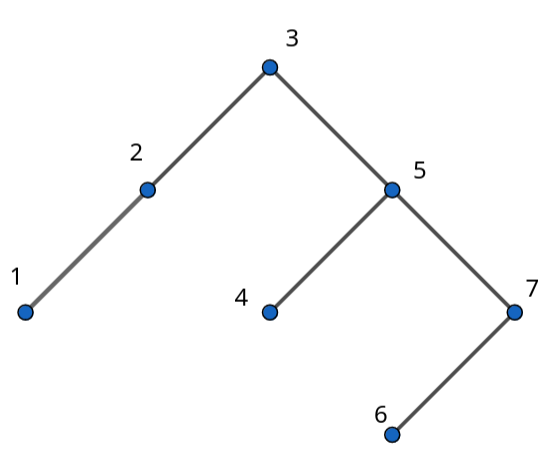
\includegraphics[scale=0.3]{./04.png}
\end{center}

Luego, accedamos a $4$ realizando \code{Zig(4)} seguido de la operación \code{Zag(4)}:

\begin{center}
  \begin{figure}[h]
    \centering
    \subfloat[Zig(4)]{
      \label{f:05}
      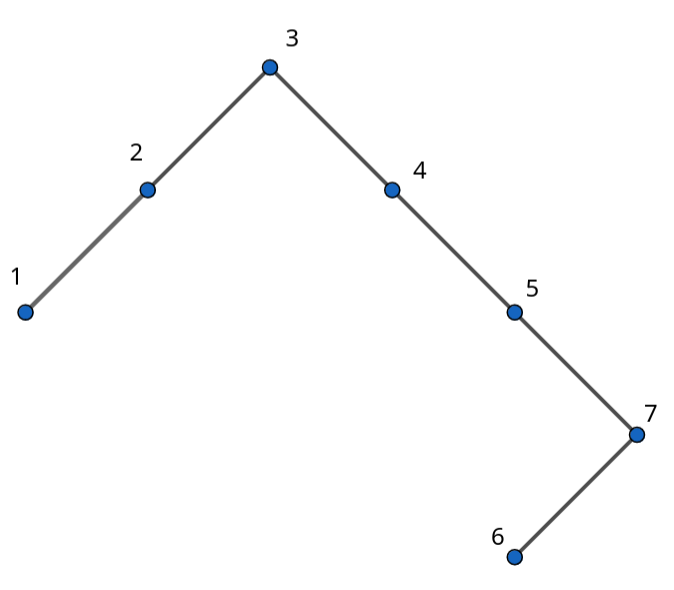
\includegraphics[width=0.4\textwidth]{05.png}}
    \subfloat[Zag(4)]{
      \label{f:06}
      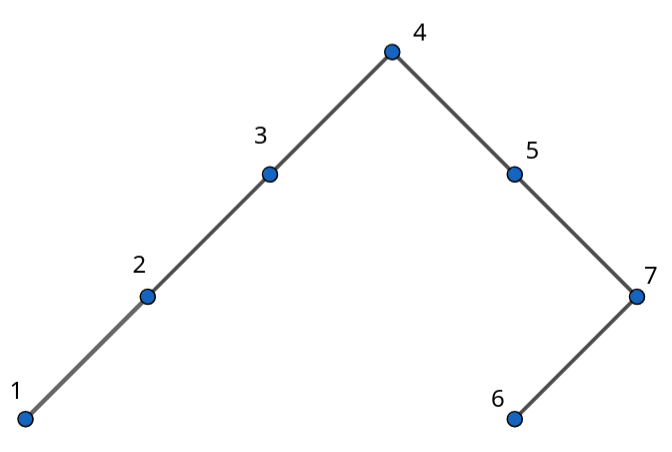
\includegraphics[width=0.4\textwidth]{06.png}}
    \caption*{Acceder a 4.}
    \label{f:animales}
  \end{figure}

  %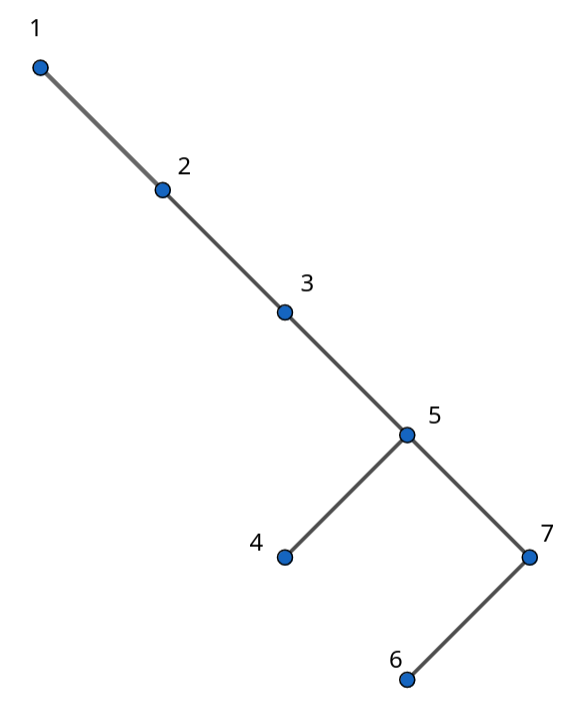
\includegraphics[scale=0.3]{./02.png}
\end{center}

Así, accedamos a $5$ realizando un \code{Zag(5)}

\begin{center}
  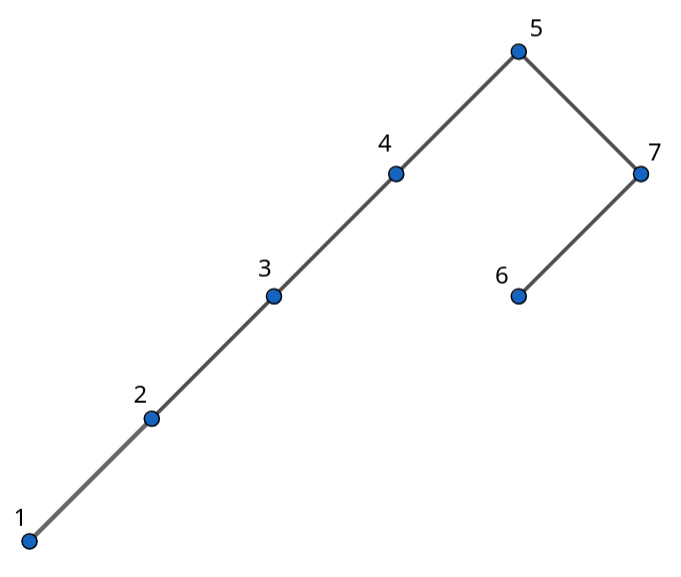
\includegraphics[scale=0.3]{./07.png}
\end{center}

\newpage
Luego, accedamos a $6$ realizando \code{Zig(6)} seguido de la operación \code{Zag(6)}:

\begin{center}
  \begin{figure}[h]
    \centering
    \subfloat[Zig(6)]{
      \label{f:08}
      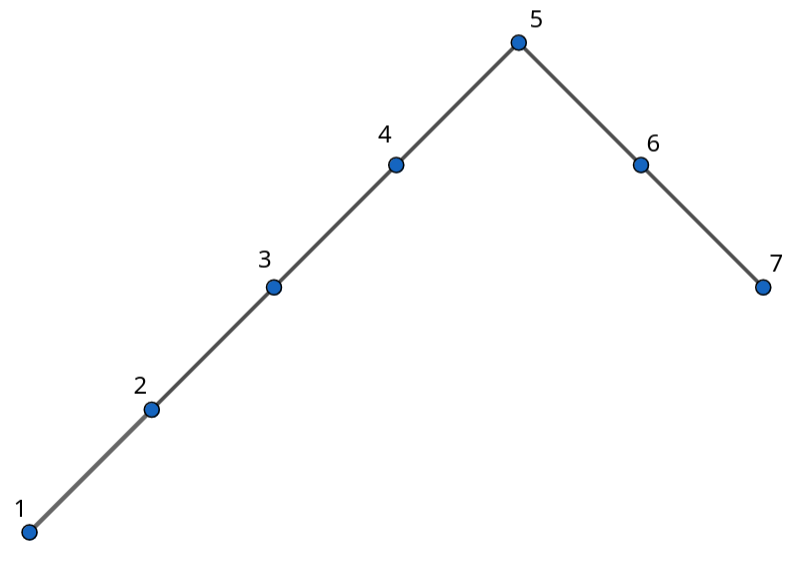
\includegraphics[width=0.4\textwidth]{08.png}}
    \subfloat[Zag(6)]{
      \label{f:09}
      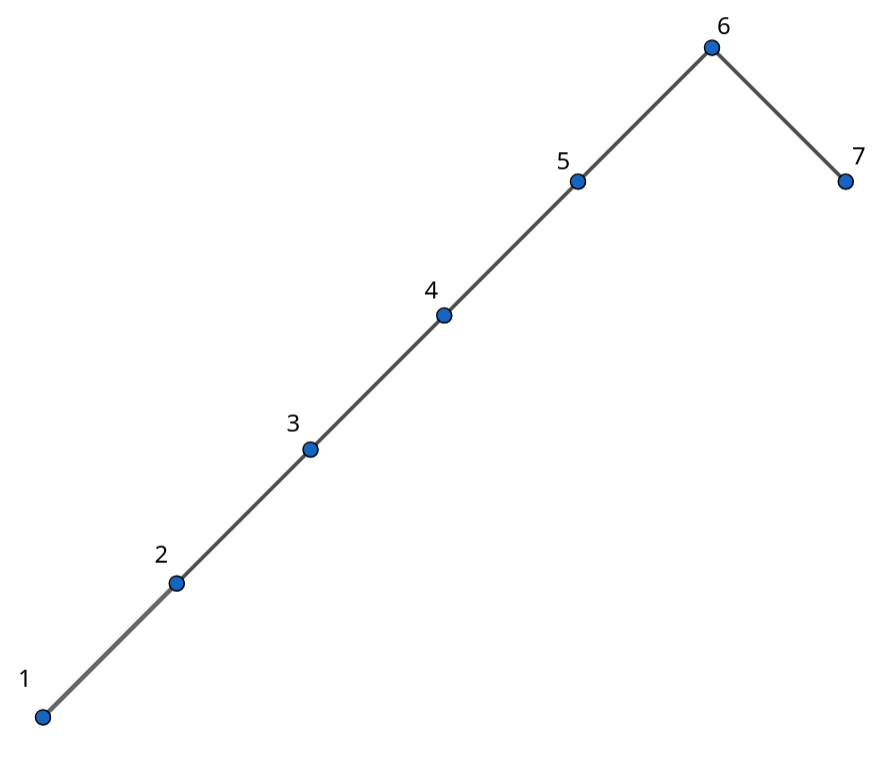
\includegraphics[width=0.4\textwidth]{09.png}}
    \caption*{Acceder a 6.}
    \label{f:animales}
  \end{figure}

  %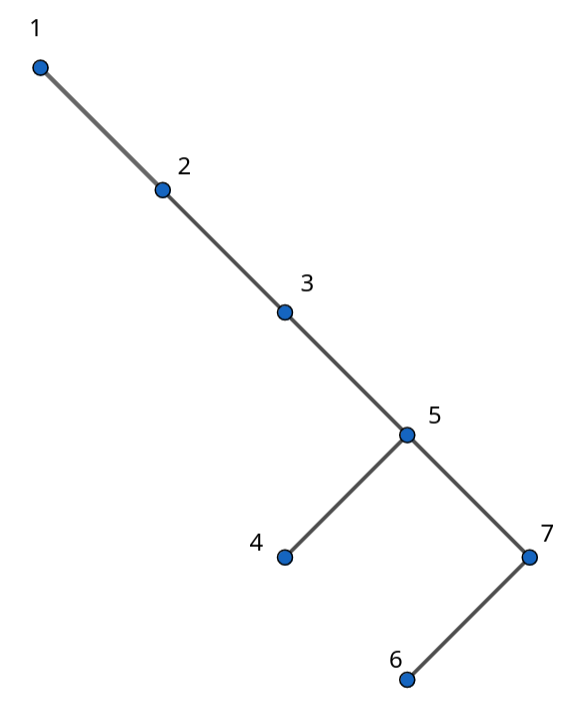
\includegraphics[scale=0.3]{./02.png}
\end{center}

Por último, accedamos a $7$ realizando un \code{Zag(7)}

\begin{center}
  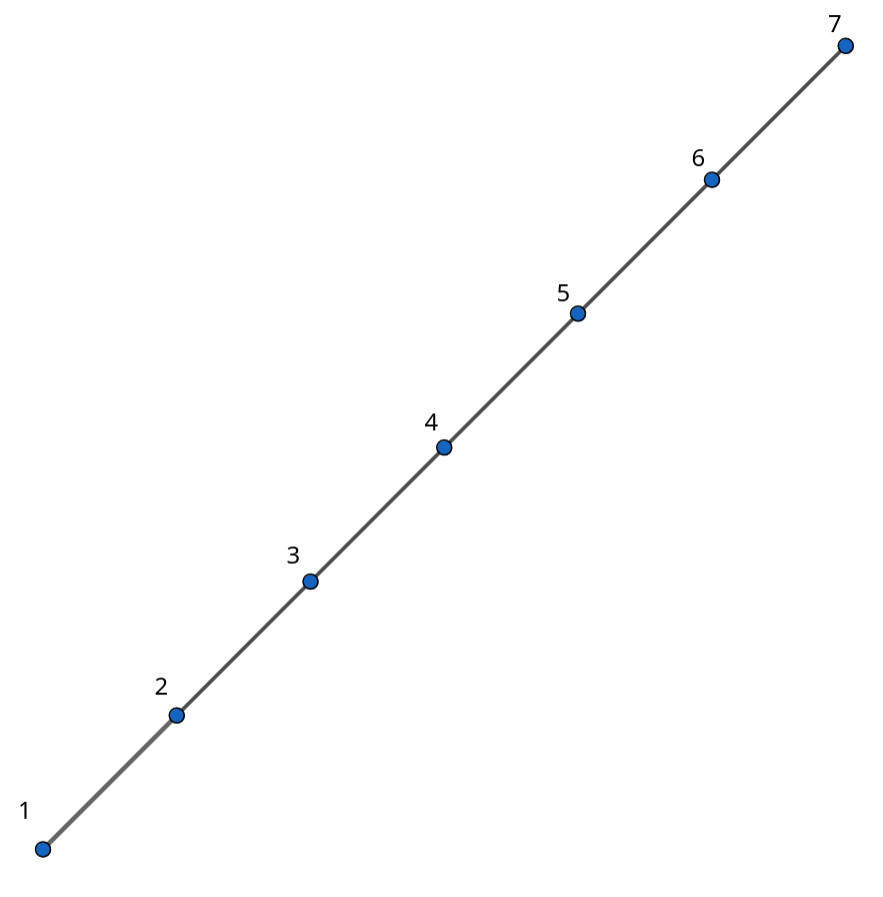
\includegraphics[scale=0.3]{./10.png}
\end{center}

Cómo podemos notar; $7 \rightarrow$ derecho, $6 \rightarrow$ izquierdo, $5 \rightarrow$ derecho,
$4 \rightarrow$ izquierdo, $3 \rightarrow$ derecho, $2 \rightarrow$ izquierdo, y por último tenemos
al $1$ que en primer instancia fue la raíz y por vacuidad podemos asumir que es un hijo derecho.\newline

De lo anterior, hemos encontrado una cadena de nodos tal que al decender por la raíz hasta la hoja se encuentran
los elementos iniciales de manera alternada entre hijos izquierdos y derechos.
\hfill $\lhd$
%\subsection*{Respuesta}

%<Tu respuesta aquí>

%\bigskip

\textbf{Pregunta 4}
%\noindent
Describe cómo modificar una \textit{skip-list} $L$ para poder realizar las siguientes dos operaciones en tiempo esperado $O(\log n)$:
\begin{itemize}
\item[$a$)] Dado un índice $i$, obtener el elemento de $L$ en la posición $i$.
\item[$b$)] Dado un valor $x$, obtener la cantidad de elementos en $L$ menores a $x$.
\end{itemize}

$\rhd$ \textbf{Solución:} Para que las operaciones anteriores sean consistentes y se mantengan
en un orden de tiempo $\mathcal{O}(\log n)$ esperados podemos mantener nuestra \textit{skip-list}
$L$ perfecta o semi-perfecta, esto implicaría un cambio de complejidad en algunas de sus operaciones
básicas y a su vez nos permitiría obtener el orden deseado en las operaciones ya mencionadas. A continuación
veamos con más detalle cómo mantener nuestra \textit{skip-list} semi-perfecta:
\begin{enumerate}
\item \textbf{Construcción.} Ordenamos nuestros valores de entrada y los posicionamos en el nivel más bajo.
  Construimos los niveles superiores tomando un valor representante por cada par de izquierda a derecha y así
  de manera recursiva hasta llegar al nivel 0, el bosquejo de la estructura quedará de la siguiente manera
  \begin{center}
    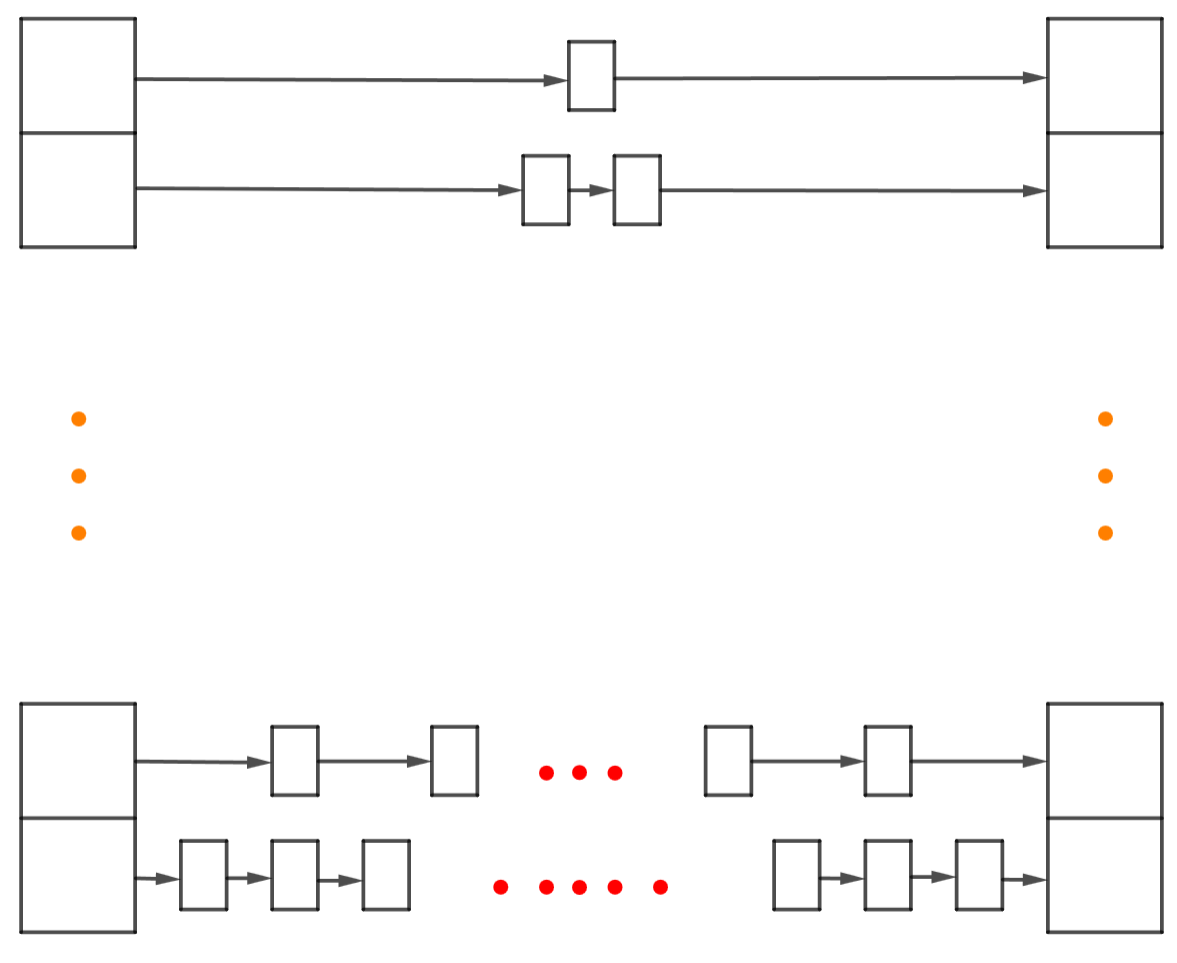
\includegraphics[scale=0.17]{./SL1.png}
  \end{center}
  estos valores tienen apuntadores para saber quién sigue en el orden, esto por cada posición en la lista original.
  Cómo es necesario mantener nuestros elementos ordenados y esto lo representamos por renglón (además de que eliminamos
  la mitad de los elementos en cada reglón de abajo hacia arriba), entonces nuestra construcción se toma
  $\mathcal{O}(n \log n)$. Además, anexaremos apuntadores de los elementos en niveles superiores a su nivel próximo inferior,
  a manera de que el elemento al que apunten sea el anterior más próximo en el orden, un bosquejo se vería de la
  siguiente manera
  \begin{center}
    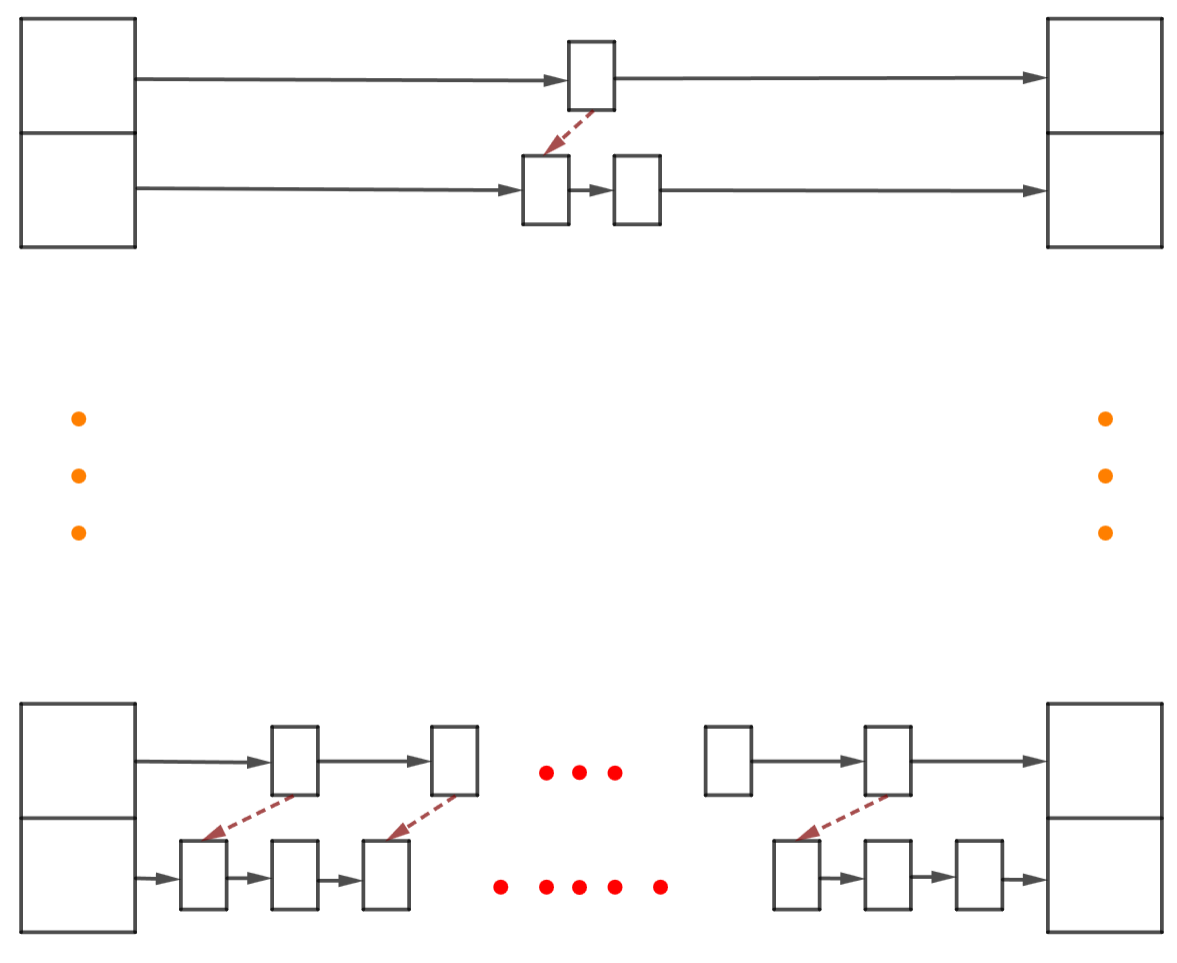
\includegraphics[scale=0.17]{./SL2.png}
  \end{center}
  notemos que esto último no nos $\mathcal{O}(n \log n)$. De la misma manera, cada nodo debe contener su respectivo índice
  suponiendo que tenemos una enumeración en el orden inicial (elementos del último nivel que están ordenado y se encuentran
  todos/completos).
\item \textbf{Insertar.} Cada vez que insertemos consultamos el número de inserciones hechas después de la
  construcción\footnote{Basta usar un contador.}, si este número es $o(n)$ respecto de los elementos originales
  entonces reconstruimos nuestra \textit{Skip-List}. Sino, entonces agregamos en el nivel 0 (de arriba hacia abajo)
  y apuntamos al anterior menor en el nivel inferior. Esto nos toma $\mathcal{O(\log n)}$ esperado (sólo cuándo
  está recién construida podemos garantizar esto), pues sólo realizamos una busqueda en el nivel 0 y en el 1 para
  encontrar su respectiva posición y apuntador.
\item \textbf{Consultar.} Debemos realizar una búsqueda desde el nivel 0, encontrar el último elemento menor al que búscamos
  consultar (o encontrar el elemento) e ir bajando por medio de sus apuntadores a sus niveles inferiores
  (de arriba hacia abajo). Esto hasta llegar al último nivel (puede que consultemos un elemento que no pertenece a $L$),
  lo que nos toma $\mathcal{O}(\log n)$ esperado.
\item \textbf{Borrar.} El borrado toma las mismas consideraciones que en el \textit{inserta} y utiliza el consulta para
  localizar el elemento y eliminar sus respectivas direcciones.
\end{enumerate}
Después de las indicaciones, observemos que
\begin{itemize}
\item[$a$)] Basta encontrar el índice del elemento en el nivel 0 y bajar en busca de su respectivo índice (esto
  gracias a que cada nodo contiene su índice y un apuntador al anterior. Esto nos toma $\mathcal{O}(\log n)$ esperado
  y sólo es exacto si $L$ no ha recibido modificaciones desde su creación.
\item[$b$)] De la misma manera que el inciso anterior, basta bajar hasta llegar al último valor mayor que $x$
  y observar su índice, digamos $i$, así sabemos que hay $i - 1$ elementos menor que $x$. Si llegamos al último
  nivel y todos los valores fueron mayores, significa que $x$ es menor respecto a los elementos de $L$ y devolvemos 0.
  Esto nos toma $\mathcal{O}(\log n)$ esperado.
\end{itemize}
  De lo anterior concluimos el ejercicio.
\hfill $\lhd$

%\subsection*{Respuesta}
%    <Tu respuesta aquí>

%\bigskip

\textbf{Pregunta 7}
Let $P$ be a set of $n$ points in the plane. The staircase of $P$ is the set of all points
in the plane that have at least one point in $P$ both above and to the right.
\begin{center}
    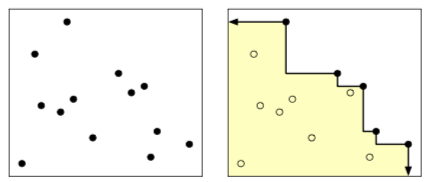
\includegraphics[scale=0.5]{escalera1}
\end{center}

\begin{enumerate}
\item Describe an algorithm to compute the staircase of a set of $n$ points in $O(n \log n)$ time.
      \newline
      
      A continuación exhibimos un algoritmo que soluciona el problema dado
      \begin{enumerate}
      \item Ordenar nuestra nube de puntos. Esto nos toma $\mathcal{O}(n \log n)$.
      \item Esta parte es un poco parecida a encontrar la envolvente convexa de una
            nube de puntos. Así,
           \begin{enumerate}
           \item Encontrar el punto $p_1$ más alto (con mayor valor respecto de $Y$). Esto nos toma $\mathcal{O}(\log n)$
                 realizando una búsqueda binaria.
           \item Encontrar el punto $p_2$ a la derecha de $p_1$ y que además sea el más alto del subconjunto de puntos
           menos $p_1$. Digamos que inicialmente $p_1$ era nuestro elemento pivotante, en este punto cambiemos nuestro
           pivote por $p_2$.
           \item Repetimos para $p_2$ y de manera iterativa, hasta no encontrar algún elemento a la derecha. 
           \end{enumerate}
           Todo esto se hace en a lo más $\mathcal{O}(n \log n)$.
      \item Ahora que tenemos una selección que formará nuestra escalera podemos construir la misma de la siguiente manera:
            \begin{enumerate}
            \item Notemos que el paso anterior nos da los puntos en el orden que deben encontrarse en nuestra escalera (descendiente).
            \item Tomemos dos puntos de nuestra selección, los más cercanos en ella (equivale a tomar los consecutivos si se guardan
            en una lista) y proyectemos al primero de manera vértical y al segundo de manera horizontal (recordar que el primer
            elemento es el más ``alto'' de todos), el corte de las proyecciones lo podemos llamar ``vértice artificial'' y así
            podemos incluir la estructura en nuestra escalera. Es decir, unimos los vértice por medio del corte formado en
            el vértice artificial.
            \item Repetimos hasta acabar con los vértices de la selección.
            \end{enumerate}
            Lo anterior nos toma a lo más $\mathcal{O}(n)$.
      \end{enumerate}
      Finalmente, devolvemos la construcción hecha en $(c)$.\newline

      \textit{Análisis de complejidad.} Podemos notar que nuestra complejidad en tiempo está contenida en
      \[\mathcal{O}(n\log n) + \mathcal{O}(n\log n) + \mathcal{O}(n) = \mathcal{O}(n\log n).\]
\item Describe and analyze a data structure that stores the staircase of a set of points, and an
  algorithm ABOVE? $(x, y)$ that returns \textsc{true} if the point $(x, y)$ is above the staircase,
  or \textsc{fals} otherwise. Your data structure should use $O(n)$ space, and your ABOVE? algorithm
  should run in $O(log n)$ time.
\end{enumerate}

\begin{center}
    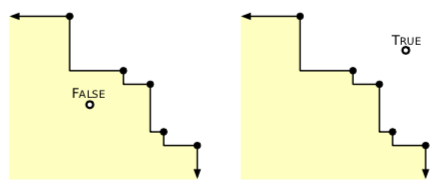
\includegraphics[scale=0.5]{escalera2}
\end{center}


  Cómo entrada tenemos nuestra escalera que es a lo más de orde $\mathcal{O}(n)$, por tanto es suficiente
  con almacenar esta para responder nuestra pregunta. ¿Cómo lo hacemos?
  \begin{itemize}
  \item La idea será similar a los árboles de segmentos.
  \item Guardamos cada segmento en un nodo.
  \item Para construir este árbol basta dividir con un ``rayo'' nuestra escalera, así vamos equilibrando nuestro árbol
  (de hecho es exactamente igual a un árbol de segmentos).
  \item \textbf{Consultar.} Basta verificar si nuestro segmento es horizontal o vértical.
  \begin{itemize}
  \item Si es horizontal basta comparar el punto $x$\footnote{Punto a comparar.} con un extremo del segmento, si
  $x$ es mayor, entonces verificamos si queda a la izquierda o derecha de nuestra escalera. Si sí regresamos TRUE, FALSE en otro caso.
  \item Si es vértical basta verificar si $x$ es mayor al extremo superior del segmento, si sí entonces verificamos si se
  encuentra a la izquierda o derecha de la escalera. Si sí, entonces devolvemos TRUE. FALSE en otro caso.
  \end{itemize}    
  \end{itemize}

Cómo basta con bajar por nuestro árbol y es un árbol binario balanceado, entonces garantizamos que la consulta se realiza en $\mathcal{O}(\log n)$.

\textbf{Pregunta 5}
Sea $S$ un conjunto de $n$ segmentos de línea sin cruces entre ellos.
Queremos responder rápidamente a consultas del tipo: dado un punto $p$
encontrar al primer segmento en $S$ por el que pasa el rayo vertical con
origen en $p$ y dirección hacia arriba. Da una estructura de datos para
resolver este problema. Acota el tiempo de consulta y el espacio requerido
por tu estructura. ¿Cuál es el tiempo de pre-procesamiento?\newline

$\rhd$ \textbf{Solución.} Para este problema utilizaremos un árbol de segmentos
modificando, dónde podamos consultar las intersecciones de la línea generada
con el resto de líneas que ya se encuentran en el árbol, entonces ¿Cómo realizamos
las consltas?\newline

1. Generamos la línea $l$ a partir de $p$, entonces consultamos las listas izquierdas y derechas
de la raíz, si la línea intersecta, al menos, un segmento entonces hemos encontrado lo deseado.\newline

2. Si la línea es menor (se encuentra a la izquierda) del nodo que estemos visitando, entonces descendemos
por el hijo izquierdo y verificamos.\newline

3. Si la línea es mayor (se encuentra a la derecha) del nodo que estemos visitando, entonces descendemos
por la derecha y verificamos.\newline

4. Si verificamos y encontramos intersecciones, entonces hemos encontrado lo deseado.\newline

5. Si descendemos hasta alguna hoja y no encontramos intersecciones, entonces no hay intersecciones y terminamos.
$\lhd$

\textbf{Pregunta 8}
En algunas aplicaciones solo nos interesa el número de puntos que caen dentro de un rango
y no reportar cada uno de ellos. En este caso nos gustaría evitar el término $O(k)$ en el tiempo de consulta.

\begin{enumerate}
\item Describe cómo un árbol de rangos de una dimensión puede adaptarse para que una consulta así se pueda
  realizar en tiempo $O(\log n)$.
\item Usando la solución al problema para una dimensión, describe cómo se pueden responder consultas de
  conteo en rangos de $d$ dimensiones en tiempo $O(\log^d n)$.
\item Describe cómo se puede usar la técnica de cascada para mejorar el tiempo de consulta en un factor
  $O(\log n)$ para dos y más dimensiones.
\end{enumerate}


$\rhd$ \textbf{Solución:} A continuación se da solución a cada uno de los incisos:
\begin{enumerate}
\item[$a$)] La versión para una dimensión sería bastante simple, y de hecho sería
  como un árbol binario de búsqueda balanceado, pues basta con preservar el árbol
  general sin los árboles ``colgados'' que tiene el árbol de búsuqeda ortogonal.
  \newline
  
  La manera de ahorrar $\mathcal{O}(k)$ durante la búsqueda de rango, sería no recorrer las
  hojas del rango encontrado. Pues, basta con realizar dos recorridos hacia abajo desde la
  raíz, uno para encontrar la cota inferior del rango y otro para encontrar la cota superior.
  Así, y por la propiedad de tener mayores a la derecha y menores a la izquierda concluimos
  que las hojas entre las seleccionadas forman parte del rango.
\item[$b$)] De la misma manera, que en el caso de una dimensión, nos ahorramos $\mathcal{O}(k)$
  al no recorrer las hojas que quedan dentro del rango. Para generalizar a $d$ dimensiones basta
  reproducir la idea de los árboles ``colgados'', pues cada nodo que no sea hoja tendrá, inicialmente
  una referencia al árbol con coordenadas en $Y$. Luego los árboles con coordenadas en $Y$ tendrán
  colgados árboles con coordenadas en $Z$, y así de manera recursiva. Cuándo se requiera obtener
  el rango bastará con bajar por el árbol principal y recorrer cada árbol asociado de manera
  recursiva para inspeccionar que efectivamente el punto quede dentro del rango requerido.
  Cómo recorremos $\log n$ el árbol principal y por cada nodo distinto a una hoja recorremos
  su árbol asociado y a su vez los asociados recursivamente, entonces tenemos una complejidad
  de $k \cdot \log n$ dónde $k = \log m \cdot \log m' \dotsm \log m^{\dotsm} \approx \log^{d - 1} n$
  y concluimos que la complejidad en general por recorrido para encontrar un punto en el rango
  es de $\mathcal{O}(\log^d n)$.\newline
  
  Como esto se tiene que hacer para el punto ``menor'' en el rango y para el punto ``mayor''
  en el rango,  entonces tenemos una complejidad contenida en
  \[2 \cdot \mathcal{O}(\log^d n) \in \mathcal{O}(\log^d n).\]
\item[$c$)] Deseamos disminuir el número de operaciones en las consultas n-dimensionales. Basta dirigir
apuntadores a rangos menores, tal cómo se usan usualmente en una dimensión. A continuación un bosquejo
ilustrativo
\begin{center}
    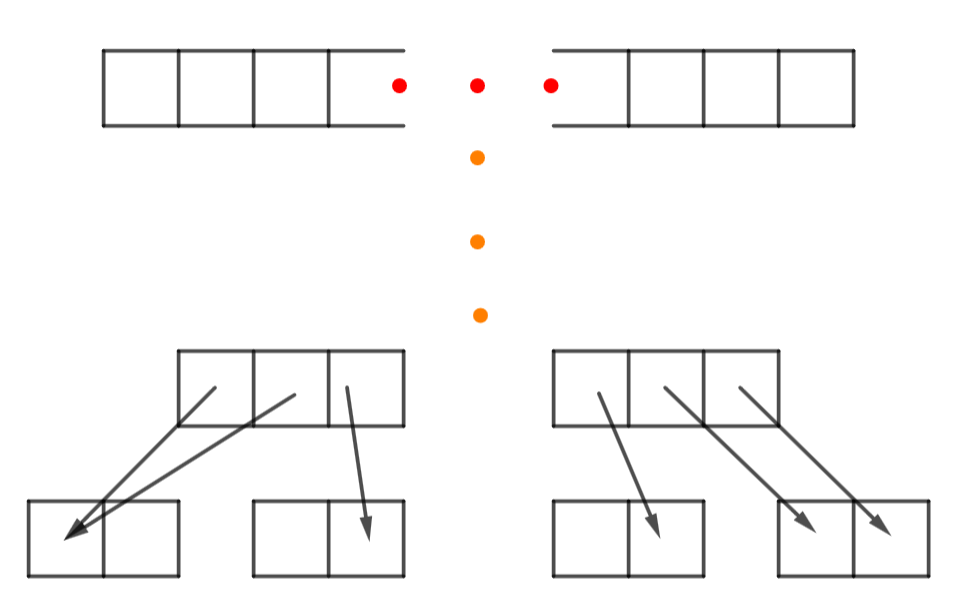
\includegraphics[scale=0.2]{Range1}
\end{center}
Sin embargo, lo anterior sólo nos funciona en una dimensión, ¿Cómo hacemos esto de manera n-dimensional?
Basta tener más apuntadores a una estructura similar que represente una segunda, tercera, ..., dimensión.
De esta manera sólo debemos descender en un árbol y buscar sus coordenadas en otros ejes sería sencillo
a través de redireccionamiento por medio de sus apuntadores. Esto es, por cada valor en el arreglo o subarreglo
debemos apuntar a su respectiva $y, z, \dotsm$ en estructuras similares. Cómo movernos por medio de estos
apuntadores es $\mathcal{O}(1)$, tenemos que la consulta se ve reducida a un orden $\mathcal{O}(\log_2 n)$.
\end{enumerate}
\hfill $\lhd$

\section*{Pregunta 9}


\noindent Diseña e implementa una versión de un Treap que incluya la operación $get(i)$, que regrese la llave con rank $i$ en el Treap. (Hint: Haz que cada nodo, $u$, mantenga un registro del tamaño del subárbol enraizado en $u$.


\subsection*{Respuesta}

<Tu respuesta aquí>

\bigskip

\section*{Pregunta 10}

\noindent Implementa un TreapList, una implementación de la interfaz lista como un Treap. Cada nodo en el Treap debería almacenar un elemento de la lista. Todas las operaciones de la Lista como $get(i)$, $set(i,x)$, $add(i, x)$ y $remove(i)$ deben tener una complejidad de $O(\log n)$ esperado.


\subsection*{Respuesta}

<Tu respuesta aquí>

\bigskip

\end{document}